\section{Computation}
\frame{\tableofcontents[currentsection]}

\begin{frame}{Computation Scale}
\begin{itemize}
    \item Number of parameters to grid should be small ($\leq 6$) to be tractable.
    \item Example designs with number of simulations and null points:
\end{itemize}
\resizebox{\linewidth}{!}{% Resize table to fit within \linewidth horizontally
\begin{tabular}{cccc} \toprule
    {Design Type} & {Number of Sims} & {Number of Null Points} & {Total Sims (billion)} \\ \midrule
    Thompson & 100,000 & 16,384 & 1.6 \\
    Exponential Hazard & 100,000 & 16,384 & 1.6 \\
    Binomial Selection & 100,000 & 262,144 & 25 \\
    Berry et al. & 10,000 & 5,308,416 & 100 \\ \bottomrule
\end{tabular}
}
\end{frame}

\begin{frame}{Computation Bottleneck}
\begin{itemize}
    \item Most of the bottleneck is in speeding up the trial simulation itself.
    \item Lots of practical designs use Bayes.
    \item Traditional methods to obtain Bayes quantity is through MCMC or analytical formulas (conjugacy).
    \item Found \emph{Integrated Nested Laplace Approximation} (INLA) to be \textbf{efficient} and \textbf{accurate}.
    \item Homegrown INLA library in development.
\end{itemize}
\end{frame}

\begin{frame}{Main Contributor of INLA Library + Application}
\begin{figure}
    \centering
    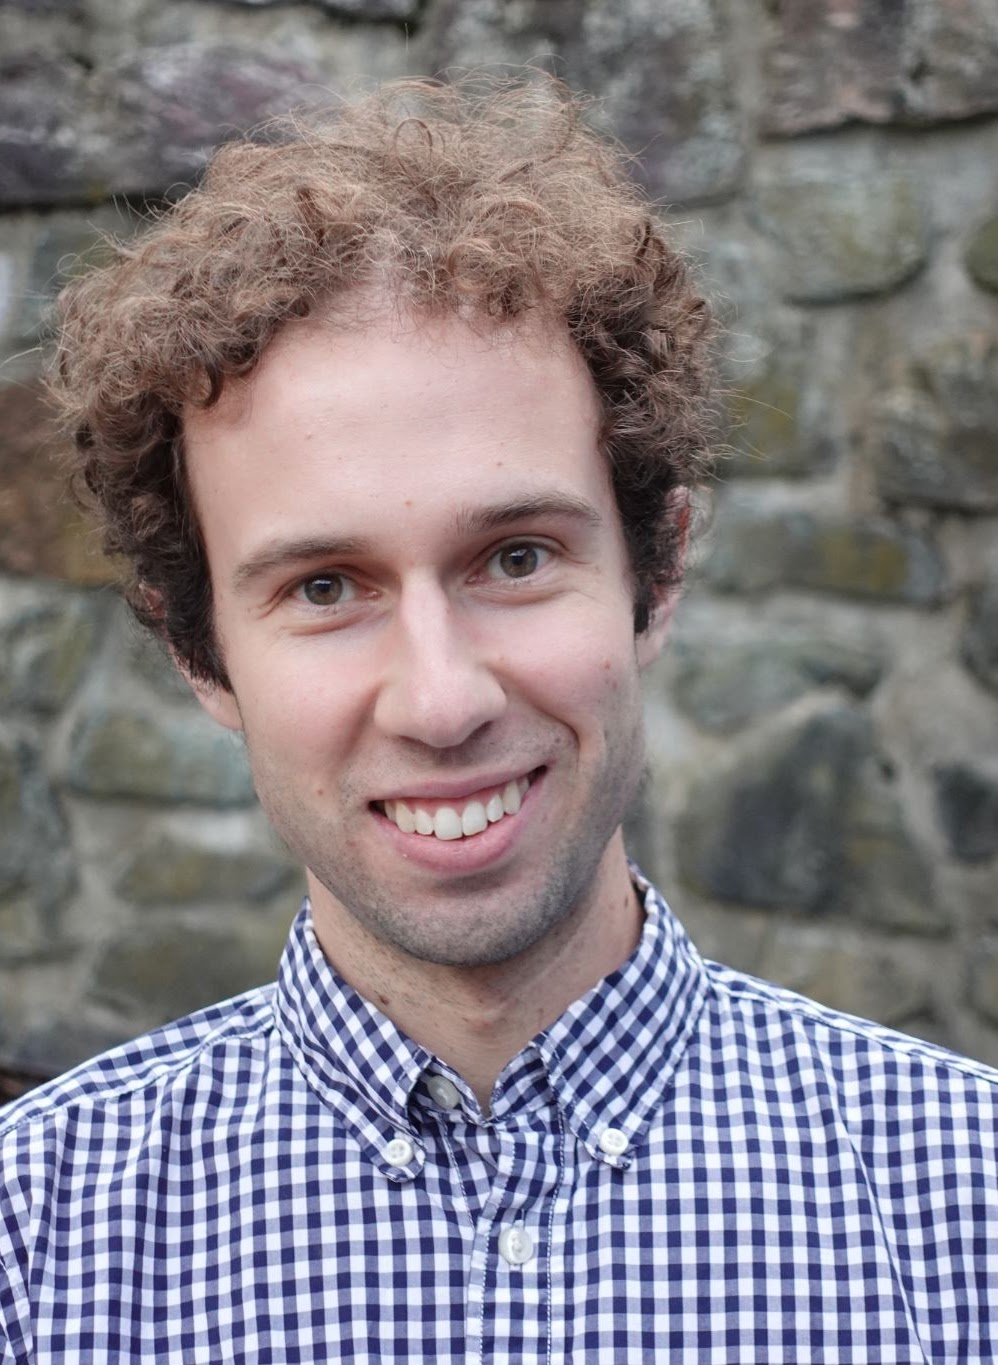
\includegraphics[width=0.4\textwidth]{figures/ben-thompson.jpeg}
    \caption{Ben Thompson}
\end{figure}
\end{frame}

\begin{frame}{Simulations are Fast!}
\begin{itemize}
    \item JAX Python library and homegrown C++ codebase.
    \item Benchmark on modern Apple M1 Macbook (CPU) and cloud machine with NVIDIA V100 (GPU):
\end{itemize}

\resizebox{\linewidth}{!}{% Resize table to fit within \linewidth horizontally
\begin{tabular}{ccccc} \toprule
    {Design Type} & {Number of Sims} & {Number of Null Points} & {Hardware} & {Time (m)} \\ \midrule
    Exponential Hazard & 100,000 & 16,384  & CPU & 1.57 \\
    Binomial Selection & 100,000 & 262,144 & CPU & 2.37 \\
    Thompson & 100,000 & 16,384 & CPU & 4 \\
    Berry et al. & 10,000 & 5,308,416 & CPU & 150 \\
    Berry et al. & 10,000 & 5,308,416 & GPU & 1.16 \\ \bottomrule
\end{tabular}
}
\end{frame}
